%! TEX program = xelatex
\documentclass{cumcmthesis}
    %\documentclass[withoutpreface,bwprint]{cumcmthesis} %去掉封面与编号页

    \title{论文题目}
    \tihao{C}            % 题号
    \baominghao{4321}    % 报名号
    \schoolname{中山大学}
    \membera{陈昊蔚}
    \memberb{李可乐}
    \memberc{蔡佳陆}
    \supervisor{指导老师}
    \yearinput{2025}     % 年
    \monthinput{9}      % 月
    \dayinput{5}        % 日

    \begin{document}
        \maketitle
        \begin{abstract}
            摘要的具体内容。
            \keywords{Spearman检验\quad  K-Means聚类分析\quad   关键词3}
        \end{abstract}
        % \tableofcontents
        \section{问题重述}
        本节旨在提取题目的关键信息,全面概括关于NIPT时点选择与胎儿异常判定的背景,
        并进一步明确根据孕妇的BMI、孕周数、孕情等个体差异,推断出既能确保准确性、又能
        尽量降低治疗窗口期缩短的风险的最佳NIPT时点以及针对女胎异常的判定方法的现实要求,
        从而更加清晰地把握问题的核心要点。

        \subsection{问题背景}
        
        进入新时代,为了响应国家“晚婚晚育、少生优生”的号召,切实提高人口素质,
        许多家庭选择在较晚的年龄生育子女。然而,随着高龄产妇比例的增加,胎儿染色体异常的风险也随之上升。
        因此,如何在孕期早期准确筛查出胎儿染色体异常,成为了产前诊断领域亟需解决的重要问题。
        \par 
        NIPT(Non-Invasive Prenatal Test,无创产前检测)是一种产前检测技术,仅需对孕妇采集血样就可检测出其中的
        胎儿游离DNA片段,并分析胎儿染色体是否存在异常(例如21号染色体数量异常导致唐氏综合征),从而在早期
        就可掌握胎儿的健康状况。NIPT技术可以有效筛查唐氏综合征、爱德华氏综合征和帕陶氏综合征这三大染色体异常疾病,
        准确率远超先前其他方法。此外,NIPT技术无需侵入性操作,避免了传统产前诊断方法可能带来的流产风险和对胎儿可能造成
        的伤害,因而被广泛应用于临床实践中。
        \par 我们本次研究的核心任务,便是基于一批孕妇的NIPT检测数据,
        构建有效的数学模型。我们希望能够借助数学模型分析胎儿Y染色体浓度和孕妇孕情的关系、不同BMI孕妇的最佳NIPT时点以及针对无Y染色体的女胎的异常判定
        方法等一系列问题。
        因此,如何利用现代数据分析与数学建模技术,排除或修正这些数据中潜在的干扰,
        准确地对上述问题完成模型建立与求解,成为了一个兼具医学意义与数据科学挑战的交叉学科课题。
        
        \subsection{基本问题}
        附件是某地区BMI偏高孕妇的NIPT检测数据,包含了孕妇的基本信息、孕情信息以及NIPT检测结果等内容。
        为了依据相关数据完成对更多孕妇的NIPT时点判断以及针对女胎的异常判定工作,现需要结合这些数据
        和已知条件,建立数学模型,分析以下问题:
        \par 
        \textbf{问题一}:依据男胎检测数据,分析胎儿Y染色体浓度与孕妇的孕周数和BMI等指标之间的相关特性,
        对有相关性的指标进行筛选,并建立数学模型,描述胎儿Y染色体浓度与孕妇孕周数和BMI等指标之间的关系。之后,再
        检验该模型的显著性。
        \par
        \textbf{问题二}:依据男胎检测数据,建立数学模型,对男胎孕妇的BMI进行分组,分析不同组别男胎孕妇的最佳NIPT时点,并
        分析检测误差对判断最佳NIPT时点的影响。
        \par
        \textbf{问题三}:依据男胎检测数据,综合考虑孕妇的身高、体重、年龄、生育次数等多种因素的影响,
        并结合检测误差以及胎儿Y染色体浓度达标比例,对孕妇的BMI进行再次分组,分析各组别孕妇的最佳NIPT时点,
        并分析检测误差对判断最佳NIPT时点的影响。
        \par
        \textbf{问题四}:依据女胎检测数据,建立数学模型,综合考虑X染色体和其他检测染色体的NIPT结果Z值、GC含量
        、读数段及相关比例、BMI等因素,分析女胎孕妇的21号、18号、13号染色体非整倍体结果,给出判断女胎是否异常的方法。
        \section{问题分析}
        \subsection{问题一分析}
        问题一要求我们依据男胎检测数据,分析胎儿Y染色体浓度与孕妇的孕周数和BMI等指标之间的相关特性。
        首先,我们需要对数据进行预处理,使得数据尽可能完整、合理。然后,我们可以使用统计分析方法,如Pearson检验和Spearman
        检验的相关系数计算和多元非线性回归分析,
        来探索胎儿Y染色体浓度与孕妇孕周数和BMI等指标之间的关系。通过建立数学模型,我们可以量化这些关系,并检验模型的显著性,以确保其可靠性。
        \par 具体步骤包括:
        \begin{itemize} 
            \item 数据预处理:清洗数据,处理缺失值和异常值。
            \item 相关性分析:计算胎儿Y染色体浓度与孕妇孕周数和BMI等指标的相关系数。
            \item 模型建立:选择合适的回归模型(如线性回归、多元回归等)来描述这些关系。
            \item 模型检验:使用统计检验方法(如F检验、t检验等)来评估模型的显著性和拟合优度。
        \end{itemize}
        \section{模型假设}
        结合题意和上述对问题的分析,为了合理简化模型的建立与求解过程,我们提出了以下假设:
        \begin{itemize}
            \item \textbf{假设1}:数据中的测量误差是随机分布的,不会系统性地偏向某一方向。
            \item \textbf{假设2}:孕妇的身体状况和生活习惯等非NIPT检测指标在研究期间保持相对稳定,不会对胎儿Y染色体浓度产生显著影响。
            \item \textbf{假设3}:不同孕妇之间的个体差异可以通过统计方法进行控制和调整。
            \item 假设4:
        \end{itemize}
        \section{符号说明}
        \begin{center}
            \begin{tabular}{cc}
                \hline
                \makebox[0.3\textwidth][c]{符号}	&  \makebox[0.4\textwidth][c]{意义} \\ \hline
                D	    & 木条宽度(cm) \\ \hline
            \end{tabular}
        \end{center}
        \section{模型的建立与求解}

        \subsection{问题一的模型建立与求解}
            \subsubsection{数据预处理}
                在进行建模之前,我们应当对附件原始数据进行合理的预处理,包括以下几个方面:
                \par
                \textbf{缺失值处理}:对于缺失的数据,采用均值填补、插值法或删除含有缺失值的样本等方法进行处理。
                \par
                \textbf{异常值检测}:使用箱线图识别BMI等变量中的异常值,并根据具体情况决定是否剔除或修正这些异常值。
                使用Python绘制BMI的箱线图,发现在上须线以上有大量异常点,在下须线以下存在一个异常点,如图1所示。
                \begin{figure}[htbp]
                \centering
                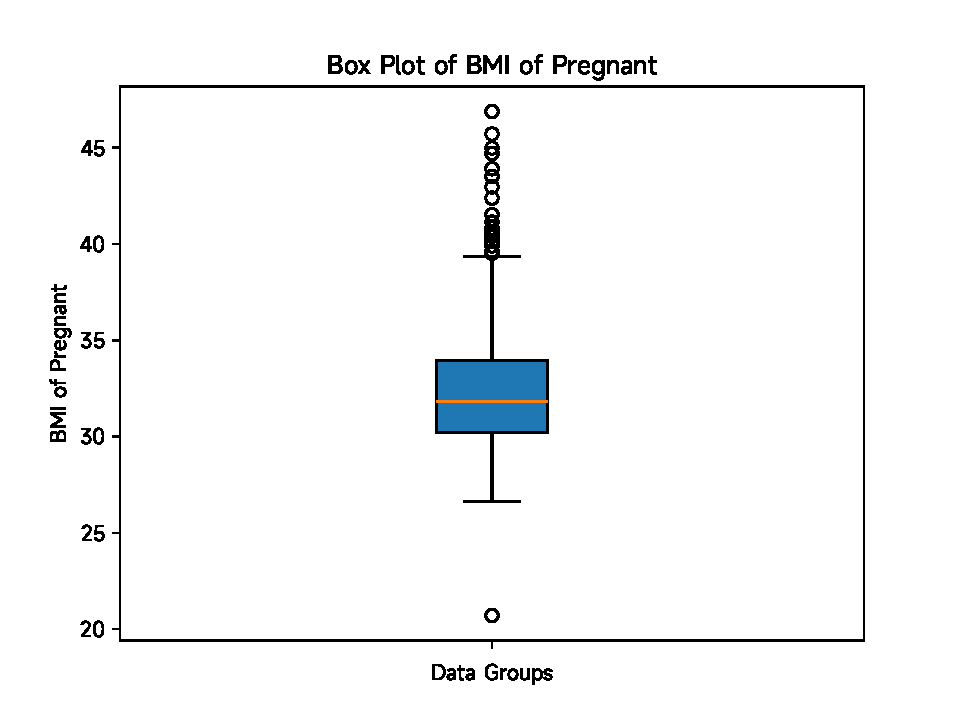
\includegraphics[width=12cm]{D:/Code/Competitions/CUMCM2025/pic/BMI箱线图.pdf}
                \caption{男胎孕妇BMI箱线图}
                \label{fi1}
                \end{figure}
                经过使用身高、体重的原始数据重新计算BMI,我们发现异常值与重新计算值的相对误差不超过$1\textperthousand$,因此对于上述异常值,我们选择保留。
                \par
                此外,对于Y染色体浓度超过$20\%$的异常值,显然已经不符合生物学常识,因此我们选择剔除这些异常值。
                \par
                \textbf{纵向数据整理}:对于“一次抽血多次检验”的数据,取其中位数作为该孕妇的最终检测结果,以减少偶然误差的影响。
                

            \subsubsection{相关性检验}
                为了分析胎儿Y染色体浓度与孕妇的孕周数和BMI等指标之间的相关特性,我们首先计算这些变量之间的相关系数。
                \par
                由于BMI和孕周数均为连续变量,我们可以使用Pearson相关系数来衡量它们与Y染色体浓度之间的线性关系。同时考虑到
                该关系也有可能是非线性的,因此我们也计算了Spearman秩相关系数,以便交互验证。
                
                \par
                然而,BMI与Y染色体浓度的Pearson相关系数仅为0.15,表明两者之间的线性关系较弱。为了进一步探讨BMI与Y染色体浓度之间可能存在的非线性关系,
                我们采用Spearman秩相关系数进行检验。计算结果显示,BMI与Y染色体浓度的Spearman相关系数为0.30,表明两者之间存在一定的单调关系。
                \par
                综合上述分析结果,我们决定在后续模型中同时考虑孕周数和BMI对Y染色体浓度的影响。
            \subsubsection{回归模型建立}
            \subsubsection{模型显著性检验}
        \subsection{问题二的模型建立与求解}
        \subsection{问题三的模型建立与求解}
        \subsection{问题四的模型建立与求解}
        \section{总结}
        \begin{thebibliography}{9}%宽度9
            \bibitem{bib:one} ....
        \end{thebibliography}
        \begin{appendices}
            附录的内容。
        \end{appendices}
\end{document}